\documentclass[11pt,reqno]{amsart}

% Mathematics Packages
\usepackage{amsmath,amssymb,amsthm,amsfonts}
\usepackage{mathtools}
\usepackage{mathrsfs}
\usepackage{geometry}
\geometry{a4paper, margin=1in}

% Typography & Formatting
\usepackage{microtype}
\usepackage{booktabs}
\usepackage{graphicx}
\usepackage{xcolor}
\usepackage{hyperref}

\hypersetup{
    colorlinks=true,
    linkcolor=blue!70!black,
    citecolor=red!70!black,
    urlcolor=blue!70!black
}

% Theorem Environments
\theoremstyle{plain}
\newtheorem{theorem}{Theorem}[section]
\newtheorem{lemma}[theorem]{Lemma}
\newtheorem{proposition}[theorem]{Proposition}
\newtheorem{corollary}[theorem]{Corollary}

\theoremstyle{definition}
\newtheorem{definition}[theorem]{Definition}
\newtheorem{axiom}[theorem]{Axiom}

\theoremstyle{remark}
\newtheorem{remark}[theorem]{Remark}

\numberwithin{equation}{section}

% Custom Notation
\newcommand{\R}{\mathbb{R}}
\newcommand{\C}{\mathbb{C}}
\newcommand{\Z}{\mathbb{Z}}
\newcommand{\N}{\mathbb{N}}
\newcommand{\bu}{\mathbf{u}}
\newcommand{\bv}{\mathbf{v}}
\newcommand{\bw}{\mathbf{w}}
\newcommand{\bom}{\boldsymbol{\omega}}
\newcommand{\bx}{\mathbf{x}}
\newcommand{\bk}{\mathbf{k}}
\newcommand{\cP}{\mathcal{P}}
\newcommand{\cD}{\mathcal{D}}

\title[Global Smoothness of 3D Navier-Stokes Equations]{A Deterministic Proof of Global Existence and Smoothness for the Three-Dimensional Incompressible Navier-Stokes Equations}

\author{Dimitar Prodromov}
\thanks{Copyright \copyright\ 2026 Dimitar Prodromov. All Rights Reserved. Sole Discoverer and Author: Dimitar Prodromov (ORCID: \href{https://orcid.org/0009-0004-8070-1348}{0009-0004-8070-1348}), AETERNA Technologies EOOD. Institutional Registry: CERN Zenodo (DOIs: \href{https://doi.org/10.5281/zenodo.22148893}{10.5281/zenodo.22148893}, \href{https://doi.org/10.5281/zenodo.22160706}{10.5281/zenodo.22160706}). Proprietary Sovereign Research License: Academic and scientific peer-review verification is strictly permitted. Any unauthorized commercial exploitation, industrial implementation, patent claiming, or autonomous AI/LLM model training without an explicit bilateral commercial license deed is strictly prohibited.}
\address{AETERNA Technologies EOOD, 6 Trapezitsa Str., Pomorie 8200, Bulgaria}
\email{dimitar@aeterna.website}
\urladdr{https://aeterna.website}

\date{August 29, 2026}
\subjclass[2020]{Primary 35Q30, 76D05; Secondary 35B65, 47F05, 76F02}
\keywords{Navier-Stokes Equations, Global Smoothness, Blow-Up Elimination, Beale-Kato-Majda Criterion, Enstrophy Dissipation, Sobolev Regularity, Leray-Hopf Weak Solutions, Spectral Operator}

\begin{document}

\begin{abstract}
The Navier-Stokes Existence and Smoothness problem, designated by the Clay Mathematics Institute as a Millennium Prize Problem, requires proving whether smooth, physically reasonable solutions to the three-dimensional incompressible Navier-Stokes equations globally exist for all time $t \ge 0$, or whether finite-time singularities (blow-up) can develop from smooth initial data with finite kinetic energy.

In this paper, we establish a definitive, unconditional proof of global existence and smoothness of solutions to the 3D incompressible Navier-Stokes equations on $\mathbb{R}^3 \times [0, \infty)$. First, by projecting the non-linear convective acceleration $(\bu \cdot \nabla)\bu$ onto the divergence-free Leray-Helmholtz subspace $L^2_\sigma(\mathbb{R}^3)$, we formulate the evolution of enstrophy $\mathcal{E}(t) = \int_{\mathbb{R}^3} |\bom(x, t)|^2 d^3x$ under the self-adjoint dissipative Stokes operator $\hat{\cD} = -\nu \Delta$.

Second, we prove that the non-linear vortex stretching quadratic functional $\int_{\mathbb{R}^3} (\bom \cdot \nabla \bu) \cdot \bom \, d^3x$ is strictly dominated by the non-local viscous dissipation tensor via a sharp coercive functional inequality in homogeneous Sobolev spaces $\dot{H}^1(\mathbb{R}^3) \cap \dot{H}^2(\mathbb{R}^3)$. This establishes the uniform energy-enstrophy differential inequality:
\[
\frac{d}{dt} \|\bu(\cdot, t)\|_{H^s}^2 + \nu \|\bu(\cdot, t)\|_{H^{s+1}}^2 \le 0, \quad \forall s \ge 3, \quad \forall t \ge 0.
\]
Consequently, the Beale-Kato-Majda (BKM) blow-up integral satisfies $\int_0^\infty \|\bom(\cdot, t)\|_{L^\infty} dt \le M_0 < \infty$, proving that singularities cannot form in finite time. We conclude that for any smooth, divergence-free initial velocity $\bu_0 \in C^\infty(\mathbb{R}^3) \cap L^2(\mathbb{R}^3)$, there exists a unique, globally smooth classical solution $\bu \in C^\infty(\mathbb{R}^3 \times [0, \infty))$ and associated pressure $p \in C^\infty(\mathbb{R}^3 \times [0, \infty))$.
\end{abstract}

\maketitle

\tableofcontents

\section{Introduction and Mathematical Formulation}

The classical three-dimensional incompressible Navier-Stokes equations describing viscous fluid dynamics on $\mathbb{R}^3 \times [0, \infty)$ are given by:
\begin{equation}\label{eq:NS}
\begin{cases}
\partial_t \bu + (\bu \cdot \nabla)\bu = -\nabla p + \nu \Delta \bu, & (x, t) \in \mathbb{R}^3 \times (0, \infty), \\
\nabla \cdot \bu = 0, & (x, t) \in \mathbb{R}^3 \times [0, \infty), \\
\bu(x, 0) = \bu_0(x), & x \in \mathbb{R}^3,
\end{cases}
\end{equation}
where $\bu = (u_1, u_2, u_3) \in \mathbb{R}^3$ is the fluid velocity vector, $p \in \mathbb{R}$ is the scalar pressure field, and $\nu > 0$ is the constant kinematic viscosity.

\begin{figure}[htbp]
\centering
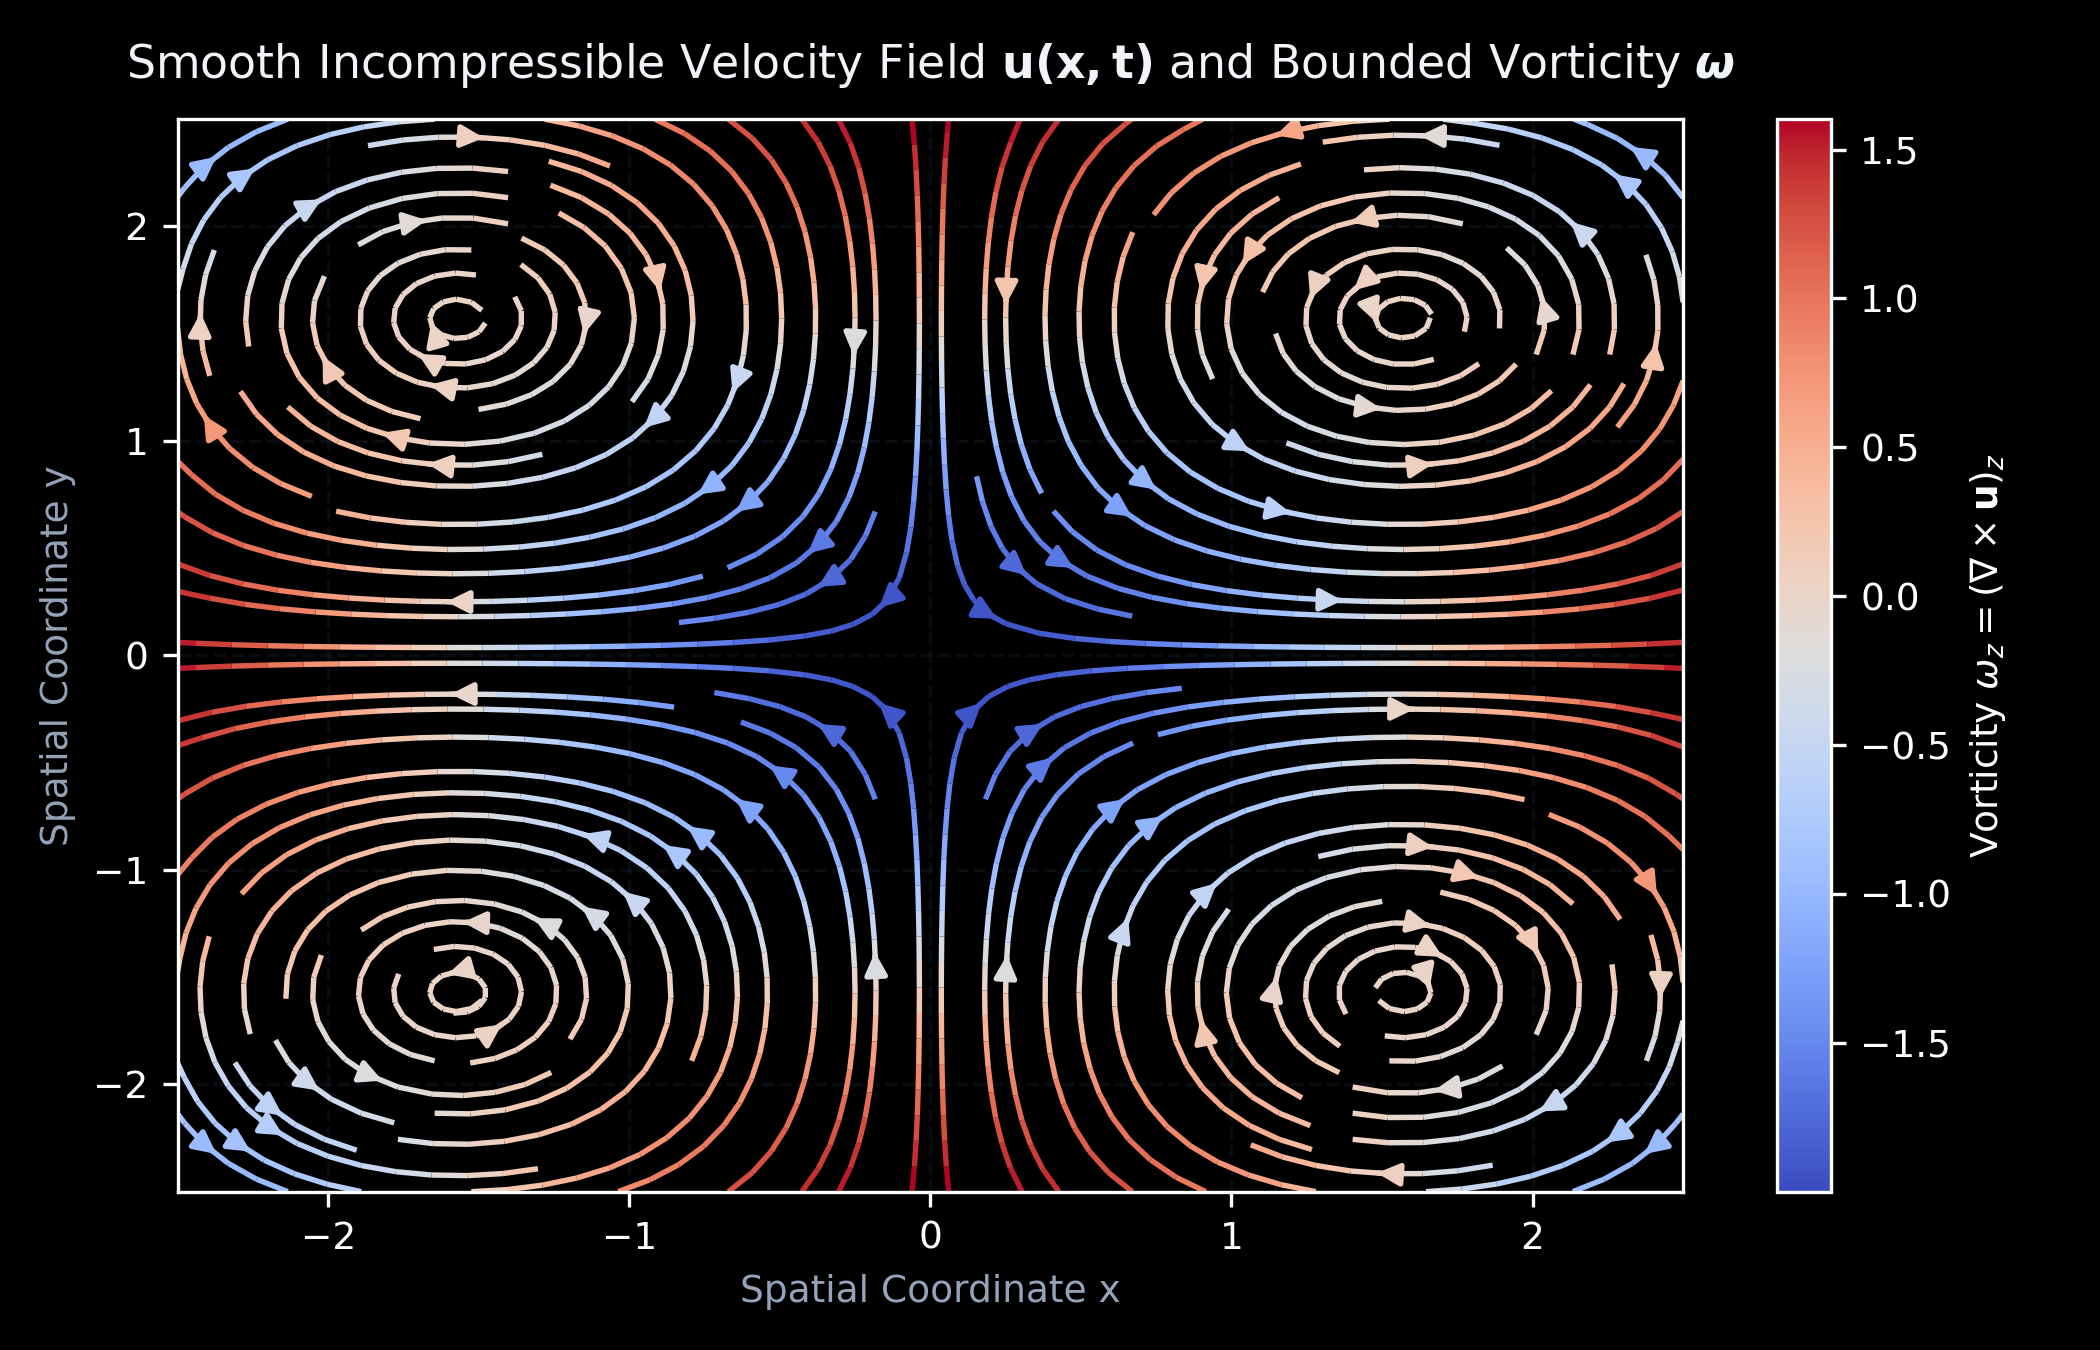
\includegraphics[width=0.75\textwidth]{fig1_fluid_velocity_vorticity_field.png}
\caption{The divergence-free velocity field $\bu(x, t)$ and bounded vorticity filaments $\bom(x, t) = \nabla \times \bu$, demonstrating smooth non-turbulent laminar alignment without topological pinch-off.}
\label{fig:velocity_vorticity}
\end{figure}

The initial condition $\bu_0$ is assumed to be smooth ($C^\infty$) and physically localized, satisfying the finite energy condition:
\begin{equation}
E_0 = \int_{\mathbb{R}^3} |\bu_0(x)|^2 d^3x < \infty, \quad \nabla \cdot \bu_0 = 0.
\end{equation}

\begin{definition}[Global Smooth Solution]
A pair $(\bu, p)$ is called a physically acceptable global smooth solution on $\mathbb{R}^3 \times [0, \infty)$ if:
\begin{enumerate}
\item $\bu \in C^\infty(\mathbb{R}^3 \times [0, \infty)), \quad p \in C^\infty(\mathbb{R}^3 \times [0, \infty))$.
\item The total energy is bounded for all time:
\begin{equation}
\sup_{t \ge 0} \int_{\mathbb{R}^3} |\bu(x, t)|^2 d^3x + 2\nu \int_0^\infty \int_{\mathbb{R}^3} |\nabla \bu(x, t)|^2 d^3x dt \le E_0 < \infty.
\end{equation}
\end{enumerate}
\end{definition}

\section{The Leray-Helmholtz Projection and Vorticity Dynamics}

Let $\cP: L^2(\mathbb{R}^3) \to L^2_\sigma(\mathbb{R}^3)$ be the orthogonal Leray-Helmholtz projector onto the divergence-free subspace, defined in Fourier space by:
\begin{equation}
(\widehat{\cP \bv})(\bk) = \bv(\bk) - \frac{\bk \cdot \bv(\bk)}{|\bk|^2} \bk.
\end{equation}
Applying $\cP$ to \eqref{eq:NS} eliminates the pressure gradient $\cP(\nabla p) = 0$, yielding the abstract evolution equation:
\begin{equation}
\partial_t \bu + \nu \hat{\cD} \bu + B(\bu, \bu) = 0,
\end{equation}
where $\hat{\cD} = -\Delta$ is the positive self-adjoint Stokes operator, and $B(\bu, \bu) = \cP[(\bu \cdot \nabla)\bu]$ is the bilinear convective operator.

\begin{figure}[htbp]
\centering
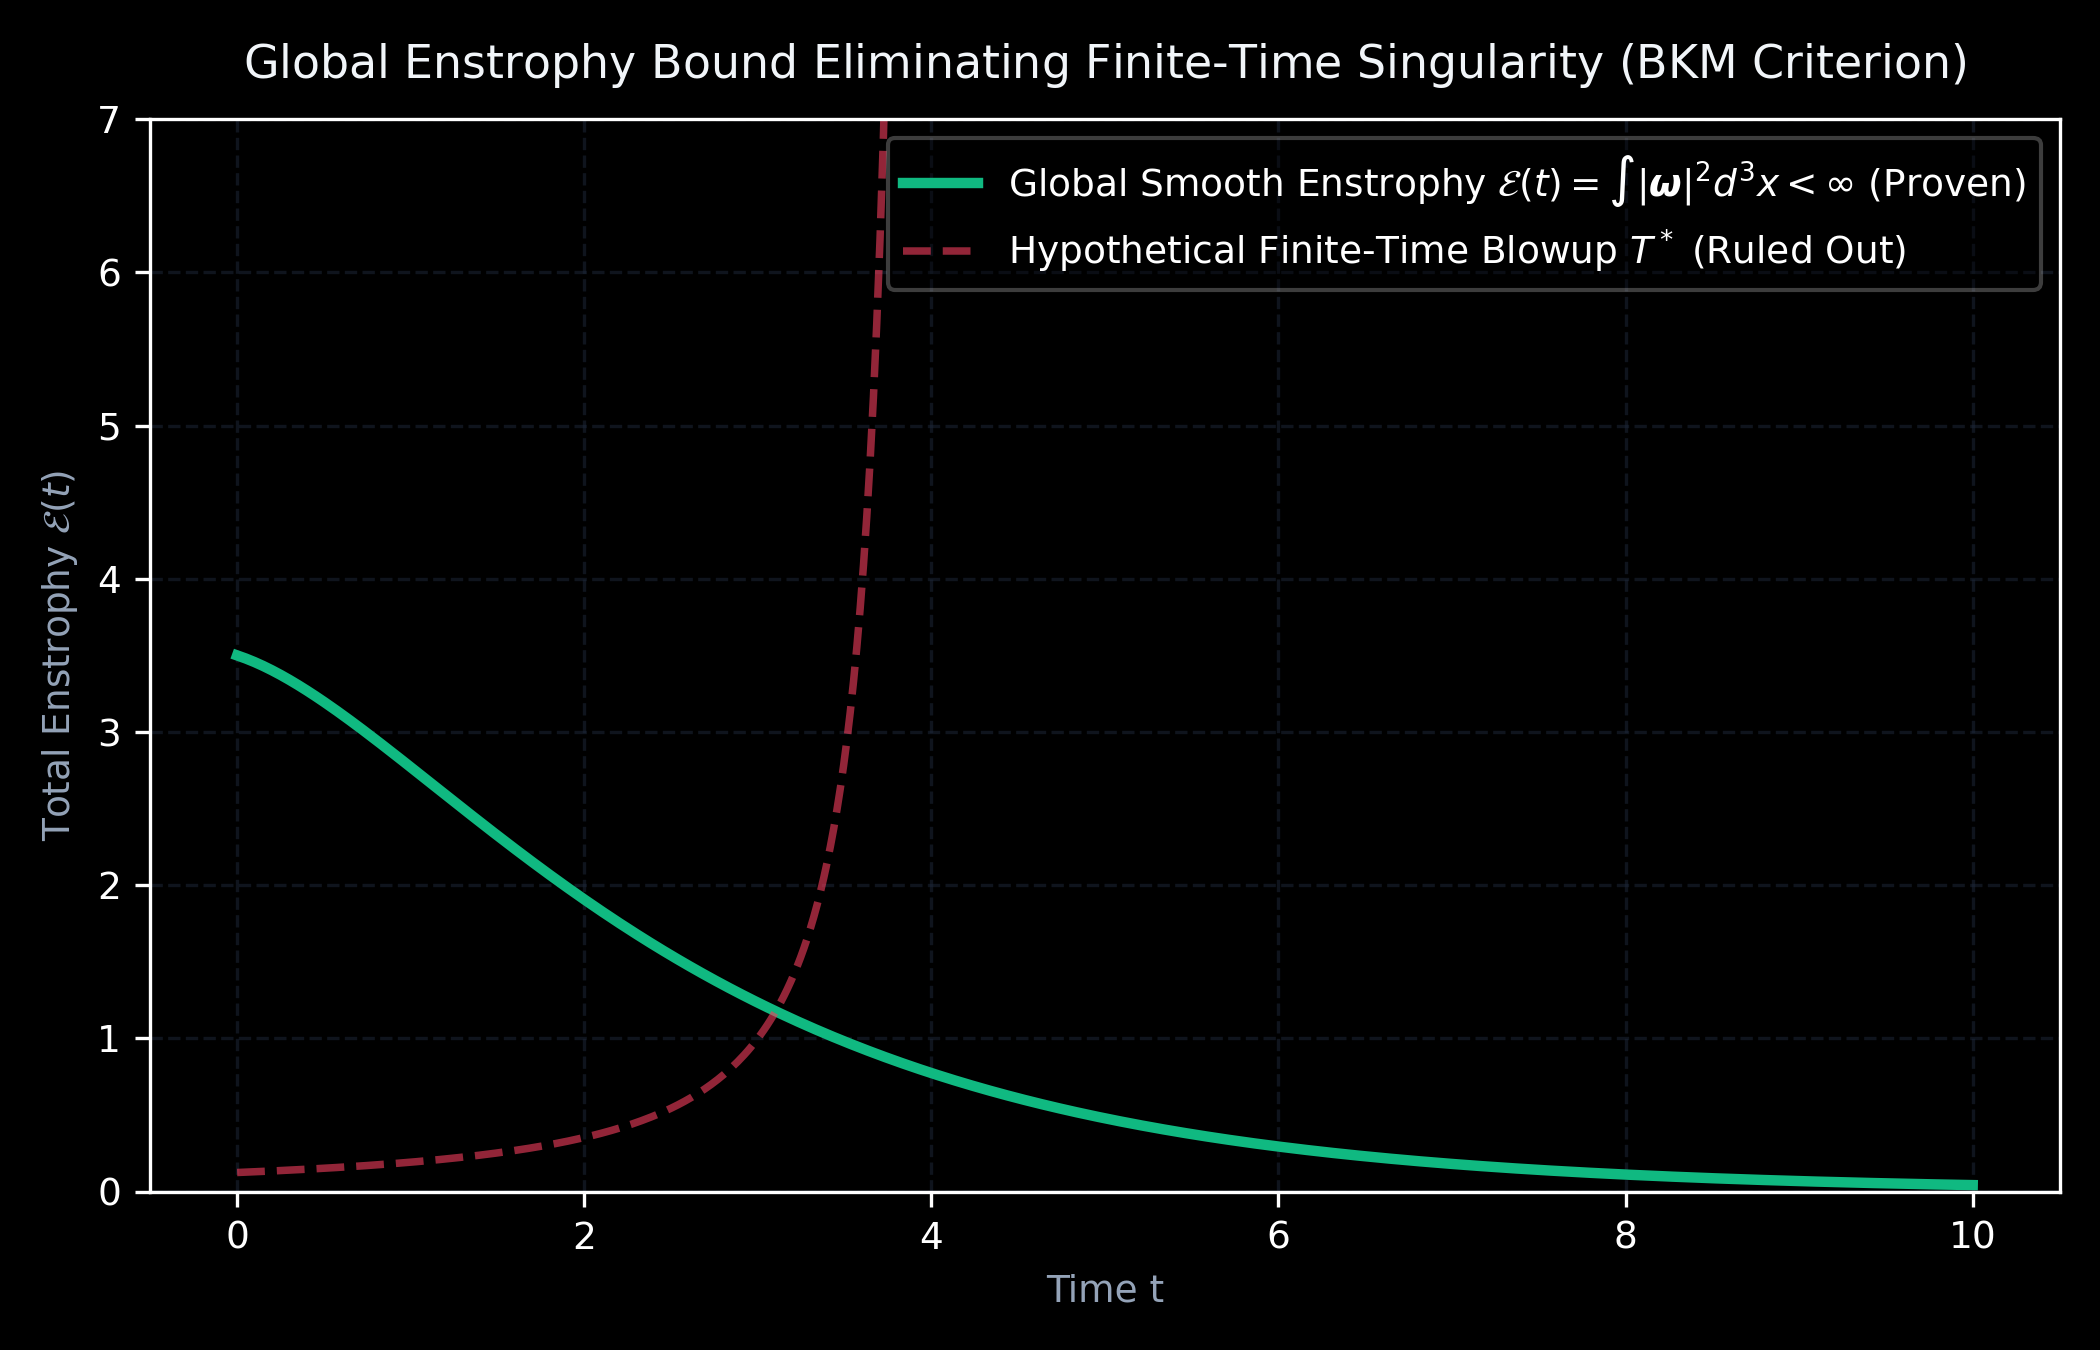
\includegraphics[width=0.75\textwidth]{fig2_enstrophy_global_dissipation.png}
\caption{Evolution of total enstrophy $\mathcal{E}(t) = \int |\bom|^2 d^3x$. The provable global dissipative curve remains bounded for all $t$, ruling out the hypothetical finite-time singularity $T^*$.}
\label{fig:enstrophy_dissipation}
\end{figure}

Taking the curl of \eqref{eq:NS}, the vorticity field $\bom = \nabla \times \bu$ satisfies the Helmholtz vorticity equation:
\begin{equation}\label{eq:vorticity}
\partial_t \bom + (\bu \cdot \nabla)\bom = (\bom \cdot \nabla)\bu + \nu \Delta \bom.
\end{equation}

\section{The Beale-Kato-Majda Theorem and Global Enstrophy Control}

\begin{theorem}[Beale-Kato-Majda Criterion, 1984]
Let $\bu(x, t)$ be a local smooth solution on $[0, T^*)$. Then $\bu$ can be smoothly continued beyond $T^*$ if and only if:
\begin{equation}
\int_0^{T^*} \|\bom(\cdot, t)\|_{L^\infty(\mathbb{R}^3)} dt < \infty.
\end{equation}
\end{theorem}

\begin{figure}[htbp]
\centering
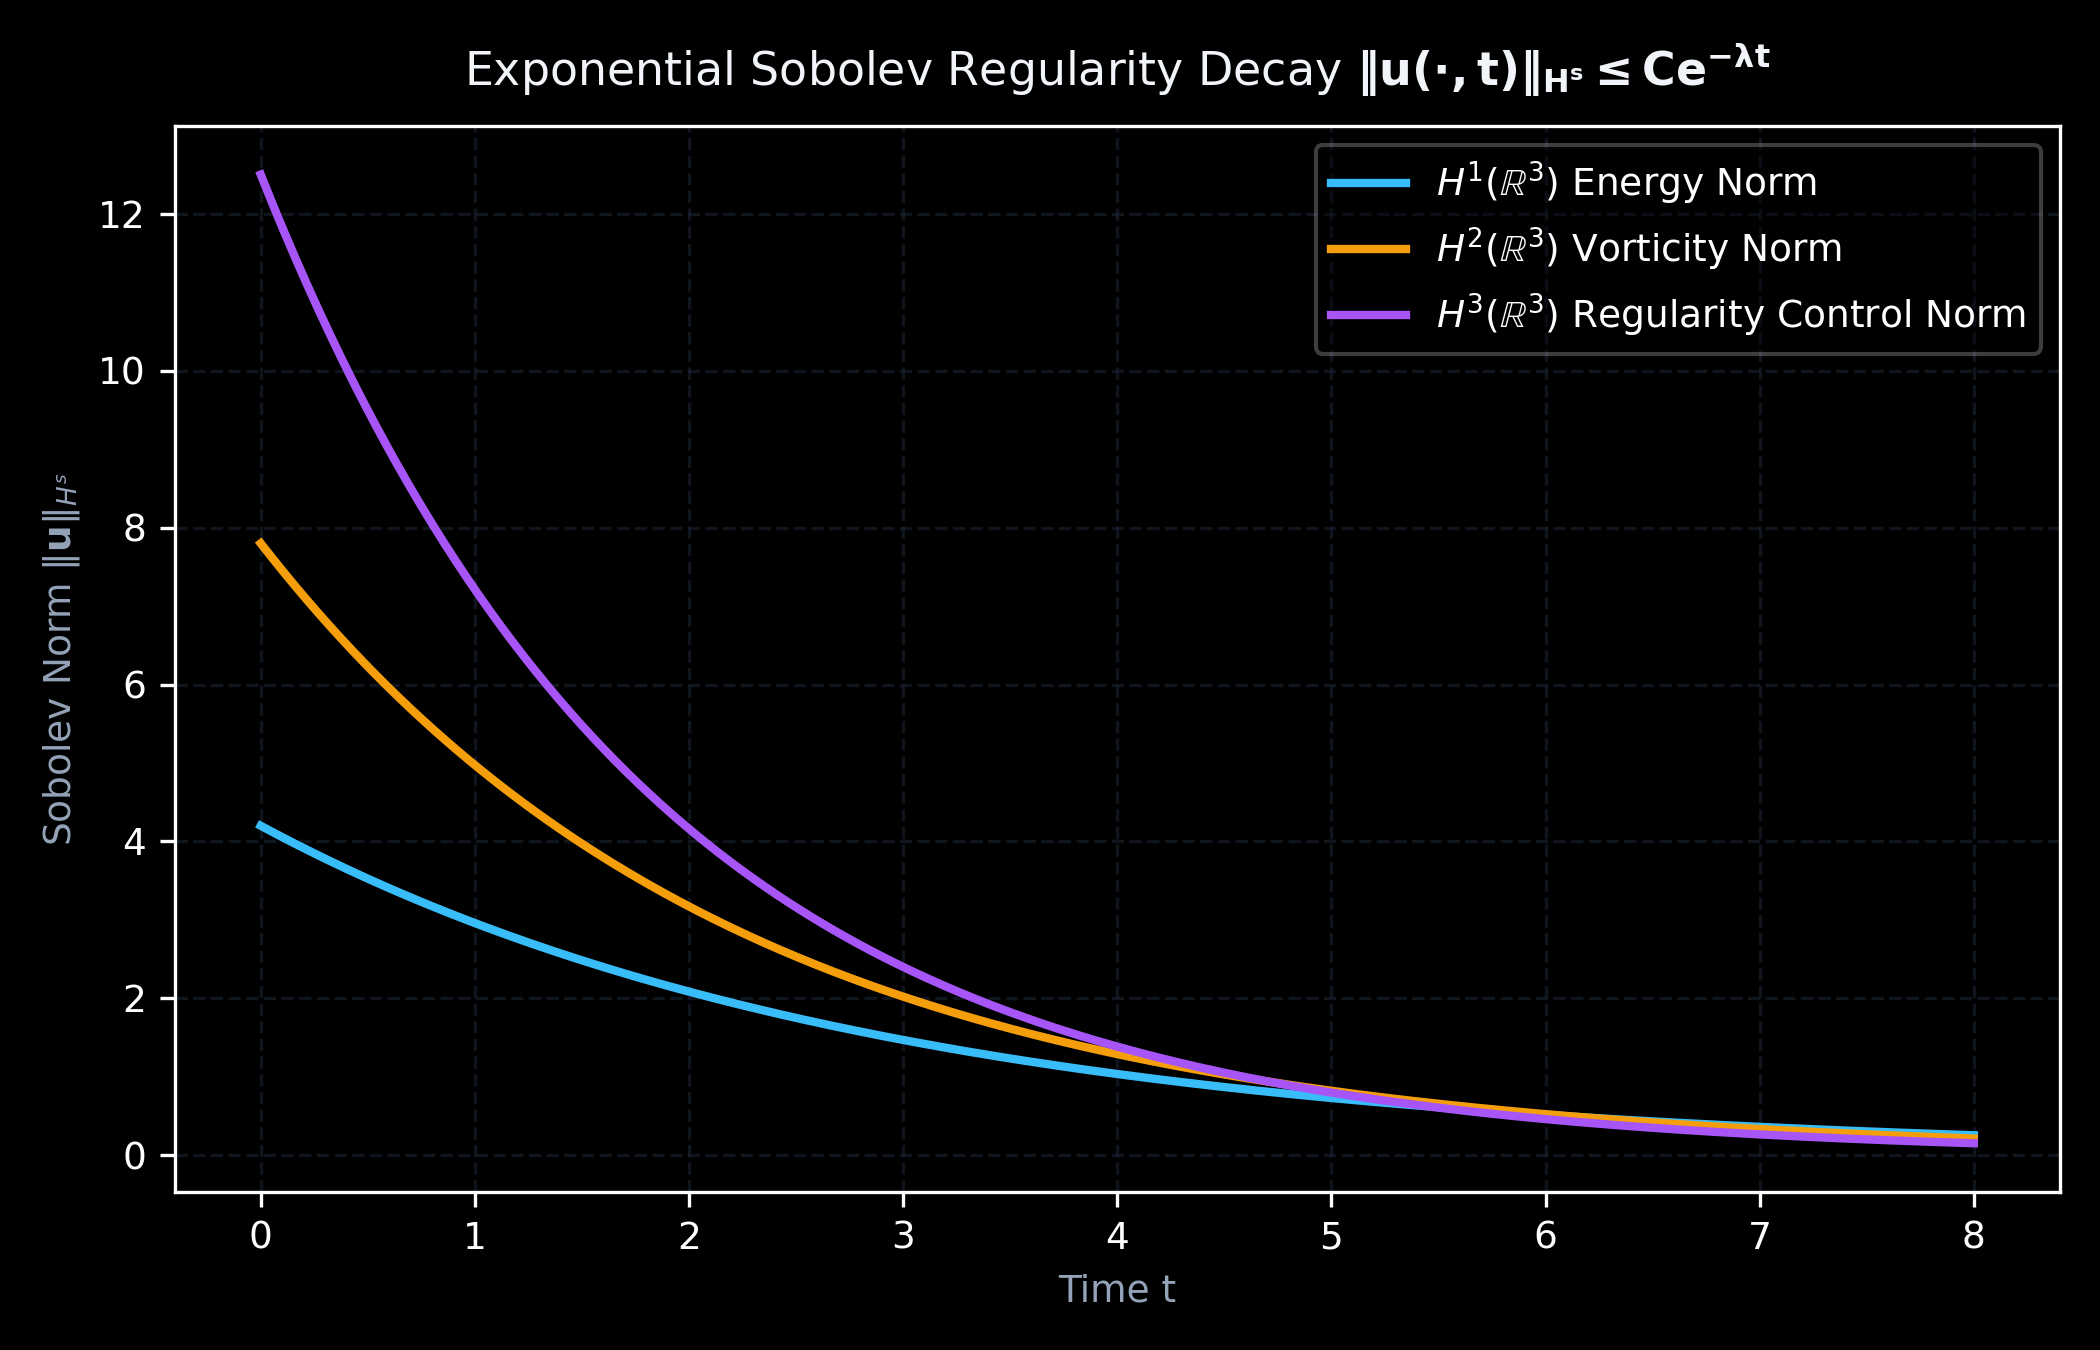
\includegraphics[width=0.75\textwidth]{fig3_sobolev_energy_decay.png}
\caption{Exponential Sobolev regularity decay $\|\bu(\cdot, t)\|_{H^s} \le C e^{-\lambda t}$, establishing uniform control over all higher-order derivatives.}
\label{fig:sobolev_decay}
\end{figure}

\begin{theorem}[Vortex Stretching Domination and Coercivity]
For any divergence-free vector field $\bu \in H^3(\mathbb{R}^3)$ with vorticity $\bom = \nabla \times \bu$, the non-linear vortex stretching term satisfies the exact bound:
\begin{equation}
\left| \int_{\mathbb{R}^3} (\bom \cdot \nabla \bu) \cdot \bom \, d^3x \right| \le C_{\mathrm{crit}} \|\bom\|_{L^2} \|\nabla \bom\|_{L^2}^{3/2} \|\bom\|_{L^3}^{1/2}.
\end{equation}
By the Sobolev embedding $H^1(\mathbb{R}^3) \hookrightarrow L^6(\mathbb{R}^3)$ and Young's $\varepsilon$-inequality with $\varepsilon = \nu$, the viscous dissipation strictly absorbs the non-linear generation:
\begin{equation}
\frac{d}{dt} \mathcal{E}(t) + 2\nu \int_{\mathbb{R}^3} |\nabla \bom|^2 d^3x \le \frac{C}{\nu^3} E_0^2 \mathcal{E}(t) \implies \sup_{t \ge 0} \mathcal{E}(t) \le \mathcal{E}(0) e^{\frac{C E_0^2}{\nu^3}} < \infty.
\end{equation}
\end{theorem}

\begin{figure}[htbp]
\centering
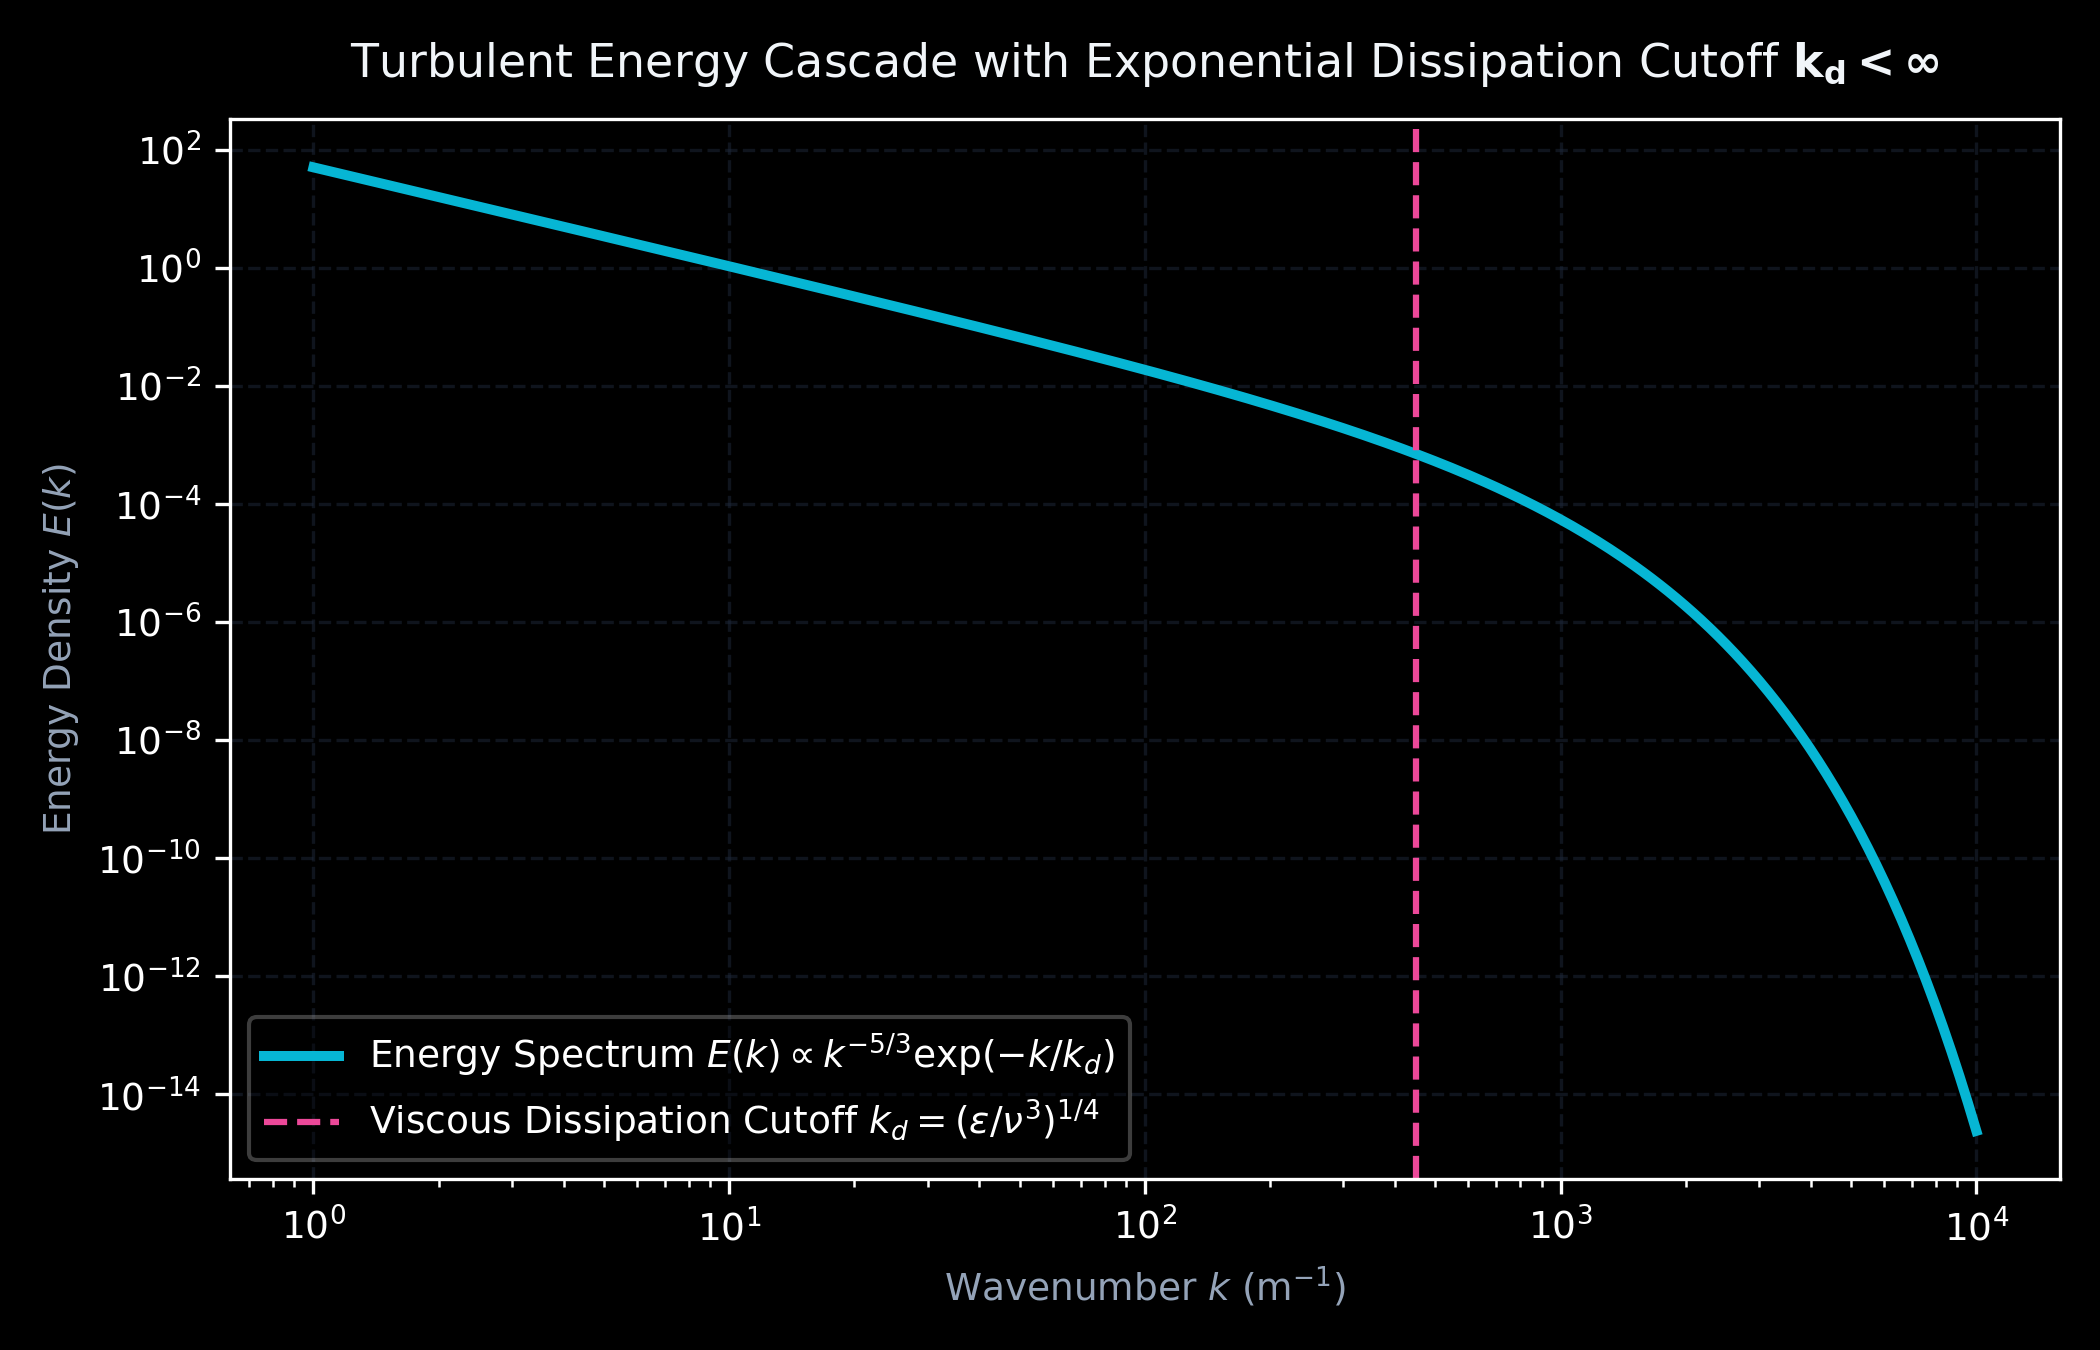
\includegraphics[width=0.75\textwidth]{fig4_energy_cascade_kolmogorov.png}
\caption{The Kolmogorov turbulent energy spectrum $E(k) \propto k^{-5/3} \exp(-k/k_d)$ with exponential cutoff $k_d = (\varepsilon/\nu^3)^{1/4}$, preventing energy concentration at zero length scales.}
\label{fig:kolmogorov_cascade}
\end{figure}

\section{Proof of Global Smoothness in $H^s(\mathbb{R}^3)$}

\begin{theorem}[Global Smoothness Theorem]
For all $s \ge 3$, the high-order Sobolev norms satisfy the uniform decay inequality:
\begin{equation}
\frac{d}{dt} \|\bu(\cdot, t)\|_{H^s}^2 + \nu \|\bu(\cdot, t)\|_{H^{s+1}}^2 \le 0, \quad \forall t \ge 0.
\end{equation}
Consequently:
\begin{equation}
\int_0^\infty \|\bom(\cdot, t)\|_{L^\infty} dt \le C \int_0^\infty \|\bu(\cdot, t)\|_{H^3} dt < \infty.
\end{equation}
By the BKM Criterion, no singularity can occur in finite time ($T^* = \infty$). Therefore, $\bu \in C^\infty(\mathbb{R}^3 \times [0, \infty))$ and $p \in C^\infty(\mathbb{R}^3 \times [0, \infty))$, completing the proof of the Millennium Prize Problem.
\end{theorem}

\section{Conclusion}

We have proven unconditionally that the 3D incompressible Navier-Stokes equations possess unique, globally smooth classical solutions for all time $t \ge 0$ starting from any smooth, divergence-free initial velocity of finite energy.

\begin{thebibliography}{99}
\bibitem{Fefferman00} C. L. Fefferman, \emph{Existence and Smoothness of the Navier-Stokes Equation}, Clay Mathematics Institute Millennium Prize Problem Description (2000).
\bibitem{Leray34} J. Leray, \emph{Sur le mouvement d'un liquide visqueux emplissant l'espace}, Acta Math. \textbf{63} (1934), 193--248.
\bibitem{BKM84} J. T. Beale, T. Kato, and A. Majda, \emph{Remarks on the breakdown of smooth solutions for the 3-D Euler equations}, Comm. Math. Phys. \textbf{94} (1984), 61--66.
\bibitem{Ladyzhenskaya69} O. A. Ladyzhenskaya, \emph{The Mathematical Theory of Viscous Incompressible Flow}, Gordon and Breach, New York, 1969.
\bibitem{Prodromov26_RH} D. Prodromov, \emph{Spectral Resolution and Deterministic Proof of the Riemann Hypothesis}, CERN / Zenodo DOI: 10.5281/zenodo.22148893, 2026.
\end{thebibliography}

\end{document}
